\chapter{Specifikacija programske potpore}
		
	\section{Funkcionalni zahtjevi}
			
			\noindent \textbf{Dionici:}
			
			\begin{packed_enum}
				
				\item Građanin
				\item Komunalni radnik			
				\item Administrator
				\item Vlasnik (naručitelj)
				\item Razvojni tim
				
				
			\end{packed_enum}
			
			\noindent \textbf{Aktori i njihovi funkcionalni zahtjevi:}
			
			
			\begin{packed_enum}
				\item  \underbar{Neregistrirani/ neprijavljeni korisnik može:}
				
				\begin{packed_enum}
					
					\item za odabrani datum na karti pregledati kontejnere 
					\item odabrati pojedini kontejner
					\begin{packed_enum}
						
						\item  pregledati popis prijava i pražnjena u tom danu
						\item  pregledati grafički prikaz prijava i pražnjenja u tom danu
						
						
					\end{packed_enum}
					\item registrirati se u sustav
					
				\end{packed_enum}
				
				
			
				\item  \underbar{Administrator može:}
				
				
				
				\begin{packed_enum}
				
					\item prijaviti se u sustav
				
				
					
						\item dodati novo kvartovsko poduzeće
						\item izbrisati postojeće kvartovsko poduzeće
						
				
				
			
					
						\item dodati novi kontejner
						\item izbrisati postojeći kontejner
				
				

				
					\item upravljati komunalnim radnicima 
						\begin{packed_enum}
					
						\item dodati novog komunalnog radnika u sustav
						\item pridodati novog komunalnog radnika kvartu
						\item premjestiti komunalnog radnika u drugi kvart
						\item izbrisati komunalnog radnika iz sustava
						
						\end {packed_enum}	
					
					
					
					
					\item prijaviti stanje kontejnera te priložiti sliku istoga
					
					\begin{packed_enum}
					
						\item prijaviti da je kontejner prazan
						\item prijaviti da je kontejner pun
						\item prijaviti da je kontejner pretrpan
						
					\end {packed_enum}	
				
					
					
				
				\end {packed_enum}	
			
				\item  \underbar{Građanin može:}
				
				\begin{packed_enum}
					
					
					\item prijaviti se u sustav
					
					
					\item prijaviti stanje kontejnera te priložiti sliku istoga
					\begin{packed_enum}
					
						\item prijaviti da je kontejner prazan
						\item prijaviti da je kontejner pun
						\item prijaviti da je kontejner pretrpan
						
					\end {packed_enum}	
					
						
				\end{packed_enum}
					
		\item  \underbar{Komunalni radnik može:}
				
				\begin{packed_enum}
					
					\item prijaviti se u sustav
					
					\item preuzeti rutu za pražnjenje kontejnera
					\item za svaki kontejner u ruti
					
						\begin{packed_enum}
						
						\item  prijaviti da je ispražnjen
						\item  prijaviti lažnu dojavu ukoliko kontejner naveden u ruti nije pun
				
					\end{packed_enum}
					
					\item prijaviti stanje kontejnera te priložiti sliku istoga
					\begin{packed_enum}
					
						\item prijaviti da je kontejner prazan
						\item prijaviti da je kontejner pun
						\item prijaviti da je kontejner pretrpan
						
					\end {packed_enum}	
					
										
				\end{packed_enum}
				
				
				\item  \underbar{Baza podataka (sudionik):}
				
				
				
				\begin{packed_enum}
				
					\item pohranjuje sve podatke o korisnicima i njihovim ovlastima
				
					\item pohranjuje sve podatke o kvartovima, kontejnerima i prijavama
					
						
				
				\end {packed_enum}	

				

				
			\end{packed_enum}
			
			\eject 
			
			
				
			\subsection{Obrasci uporabe}
				
			
					

					\noindent \underbar{\textbf{UC01-Registracija}}
					\begin{packed_item}
	
						\item \textbf{Glavni sudionik: } Neregistrirani korisnik
						\item  \textbf{Cilj:} Stvaranje korisničkog računa za pristup sustavu
						\item  \textbf{Sudionici:} Baza podataka
						\item  \textbf{Preduvjet:} -
						\item  \textbf{Opis osnovnog tijeka:}
						
						\item[] \begin{packed_enum}
	
							\item Korisnik odabire registraciju u sustav
							\item Korisnik unosi ime, prezime, email i lozinku
							\item Korisnik dobiva obavijest o uspješnoj registraciji u sustav
						\end{packed_enum}
						
						\item  \textbf{Opis mogućih odstupanja:}
						
						\item[] \begin{packed_item}
	
	
						\item[2.a] Email je prethodno već zauzet
							
							\item[] \begin{packed_enum}
								
								\item Sustav obavještava korisnika da unese mail koji ne postoji u sustavu
								\item Korisnik ponovno unosi podatke ili odustaje od registracije
								
							\end{packed_enum}
							\item[2.b] Unos neispravnog emaila
							
							\item[] \begin{packed_enum}
								
								\item Sustav obavještava korisnika da je unio neispravan podatak
								\item Korisnik ponovno unosi podatke ili odustaje od registracije
								
							\end{packed_enum}
							\item[2.c] Korisnik je unio manje od osam znakova za lozinku
							
								\item[] \begin{packed_enum}
								
								\item Sustav obavještava korisnika da je unio neispravan podatak
								\item Korisnik ponovno unosi podatke ili odustaje od registracije
								
							\end{packed_enum}
							
						\end{packed_item}
					\end{packed_item}
					
					
					\noindent \underbar{\textbf{UC02-Prijava u sustav}}
					\begin{packed_item}
	
						\item \textbf{Glavni sudionik: } Građanin, komunalni radnik, administrator
						\item  \textbf{Cilj:} Mogućnost pristupa korisničkom sučelju
						\item  \textbf{Sudionici:} Baza podataka
						\item  \textbf{Preduvjet:} Registracija
						\item  \textbf{Opis osnovnog tijeka:}
						
						\item[] \begin{packed_enum}
	
							\item Korisnik unosi korisničko email i lozinku
							\item Sustav vraća poruku o ispravnosti unesenih podataka
							\item Sustav korisniku omogućava pristup korisničkim funkacijama 
						\end{packed_enum}
						
						\item  \textbf{Opis mogućih odstupanja:}
						
						\item[] \begin{packed_item}
	
							\item[2.a] Unos neispravnog emaila ili lozinke
							
							\item[] \begin{packed_enum}
								
								\item Sustav obavještava korisnika da je unio neispravan podatak i vraća korisnika u korak 1.
								
							\end{packed_enum}
													
						\end{packed_item}
					\end{packed_item}


		\noindent \underbar{\textbf{UC03-Dodaj najkorištenije kontejnere}}
					\begin{packed_item}
	
						\item \textbf{Glavni sudionik: } Građanin, komunalni radnik, administrator
						\item  \textbf{Cilj:} Brži pristup kontejner koje su predmet česte uporabe
						\item  \textbf{Sudionici:} Baza podataka
						\item  \textbf{Preduvjet:} Korisnik je prijavljen u sustav
						\item  \textbf{Opis osnovnog tijeka:}
						
						\item[] \begin{packed_enum}
	
							\item Korisnik odabire traženi kontejner na karti
							\item Sustav prikazuje opcije vezane za odabrani kontejner
							\item Korisnik odabire i označava opciju "omiljeni kontejner"
							\item Sustav sprema unesenu promjenu
						\end{packed_enum}
						
						
					\end{packed_item}
					
					
					
					
	\noindent \underbar{\textbf{UC04-Ukloni iz najkorištenijih}}	
				\begin{packed_item}
	
						\item \textbf{Glavni sudionik: }Građanin, komunalni radnik, administrator
						\item  \textbf{Cilj:} Povećanje preglednosti karte i lakša uporaba iste
						\item  \textbf{Sudionici:} Baza podataka
						\item  \textbf{Preduvjet:} Korisnik je prijavljen u sustav
						\item  \textbf{Opis osnovnog tijeka:}
						
						\item[] \begin{packed_enum}
	
							\item Korisnik odabire traženu kantu na karti
							\item Sustav prikazuje opcije vezane za odabrani kontejner
							\item Korisnik odabire i označava opciju "ukloni iz omiljenih kontejnera"
							\item Sustav sprema unesenu promjenu
						\end{packed_enum}
						
					\end{packed_item}


	\noindent \underbar{\textbf{UC05-Preuzimanje rute}}
					\begin{packed_item}
	
						\item \textbf{Glavni sudionik: } Komunalni radnik
						\item  \textbf{Cilj:} Preuzimanje optimalne putanje za pražnjenje kanti
						\item  \textbf{Sudionici:} Baza podataka
						\item  \textbf{Preduvjet:} Korisnik je prijavljen u sustav
						\item  \textbf{Opis osnovnog tijeka:}
						
						\item[] \begin{packed_enum}
	
							\item Korisnik odabire preuzimanje rute
							\item Sustav prikazuje popis kontejnera za pražnjenje
							\item Korisnik pokreće rutu
						\end{packed_enum}
						
						\item  \textbf{Opis mogućih odstupanja:}
						
						\item[] \begin{packed_item}
	
							\item[1.a] Nedostatan broj kontejnera spremnih za pražnjenje 
							
							\item[] \begin{packed_enum}
								
								\item Sustav javlja da nema dovoljan broj kontejnera za stvoriti rutu i vraća korisnika u korak 1
								
							\end{packed_enum}
														
						\end{packed_item}
					\end{packed_item}


	\noindent \underbar{\textbf{UC06-Potvrda pražnjenja}}
					\begin{packed_item}
	
						\item \textbf{Glavni sudionik: }Komunalni radnik
						\item  \textbf{Cilj:} Potvrda pražnjenja kanti s rute
						\item  \textbf{Sudionici:} Baza podataka
						\item  \textbf{Preduvjet:} Korisnik je prijavljen i pokrenuo je rutu (UC05)
						\item  \textbf{Opis osnovnog tijeka:}
						
						\item[] \begin{packed_enum}
	
							\item Korisnik odabire kontejner iz rute
							\item Sustav prikazuje opcije vezane za odabrani kontejner
							\item Korisnik označava da je kontejner ispražnjen
							\item Sustav sprema unesenu promjenu
							
						\end{packed_enum}
						
						\item  \textbf{Opis mogućih odstupanja:}
						
						\item[] \begin{packed_item}
	
							\item[3.a] kontejner nije pun
							
							\item[] \begin{packed_enum}
								
								\item Korisnik označava da je dojava lažna
								\item Sustav prikazuje sljedeći kontejner iz rute
								
							\end{packed_enum}
						\end{packed_item}
					\end{packed_item}

	\noindent \underbar{\textbf{UC07-Dodavanje komunalnog radnika}}
					\begin{packed_item}
	
						\item \textbf{Glavni sudionik: }Administrator
						\item  \textbf{Cilj:} Stvaranje korisničkog računa za novog korisnika
						\item  \textbf{Sudionici:} Baza podataka
						\item  \textbf{Preduvjet:} Korisnik je prijavljen u sustav
						\item  \textbf{Opis osnovnog tijeka:}
						
						\item[] \begin{packed_enum}
	
							\item Korisnik odabire kvart
							\item Sustava prikazuje popis radnika u odabranom kvartu
							\item Korisnik odabire stvaranje novog radnika u odabranom kvartu
							\item Sustav otvara formu za registraciju novog radnika
							\item Korisnik unosi podatke o novom radniku
							\item Sustav sprema unesenu promjenu
						\end{packed_enum}
						
						\item  \textbf{Opis mogućih odstupanja:}
						
						\item[] \begin{packed_item}
	
							\item[3.a] U odabranom kvartu ima previše radnika 
							
							\item[] \begin{packed_enum}
								
								\item Sustav obavještava korisnika da nije moguće unijeti novog radnika i vraća ga u korak 2
								
							\end{packed_enum}
							\item[5. a] Korisnik je unio neispravne podatke o novom radniku 
							
								\item[] \begin{packed_enum}
								
								\item Sustav upozorava na pogrešku pri unosu i vraća korisnika u korak 4
								
							\end{packed_enum}
							
							\item[5. a] Korisnik je pokušao stvoriti novog radnika koji već postoji u sustavu
							
								\item[] \begin{packed_enum}
								
								\item Sustav javlja kako radnik već postoji i vraća korisnika u korak 2
								
							\end{packed_enum}

							
						\end{packed_item}
					\end{packed_item}

	\noindent \underbar{\textbf{UC08-Premještanje komunalnog radnika}}
					\begin{packed_item}
	
						\item \textbf{Glavni sudionik: }Administrator
						\item  \textbf{Cilj:} Premještanje komunalnog radnika iz jedne kvartovske podružnice u drugu
						\item  \textbf{Sudionici:} Baza podataka
						\item  \textbf{Preduvjet:} Korisnik je prijavljen u sustav
						\item  \textbf{Opis osnovnog tijeka:}
						
						\item[] \begin{packed_enum}
	
							\item Korisnik odabire kvart u kojem se trenutno nalazi traženi radnik
							\item Sustav prikazuje popis radnika u odabranom kvartu
							\item Korisnik odabire traženog radnika 
							\item Sustav prikazuje podatke o odabranom radniku
							\item Korisnik mijenja kvart kojem je radnik pridjeljen
							\item Sustav sprema unesenu promjenu
						\end{packed_enum}
						
						\item  \textbf{Opis mogućih odstupanja:}
						
						\item[] \begin{packed_item}
	
							\item[5.a] Prevelik broj radnika u ciljanom poduzecu
							
							\item[] \begin{packed_enum}
								
								\item Sustav obavještava korisnika o nemogućnosti izvršavanja tražene akcije i vraća korisnika u korak 4
								
								
							\end{packed_enum}
							\item[5.b] Premalo radnika u početnom kvartu
							
								\item[] \begin{packed_enum}
								
								\item Sustav obavještava korisnika o nemogućnosti izvršavanja tražene akcije i vraća korisnika u korak 4
								
								
							\end{packed_enum}
							
						\end{packed_item}
					\end{packed_item}

				
				
					
				
				
					
				
				
					\noindent \underbar{\textbf{UC09-Prijava praznog kontejnera}}
					\begin{packed_item}
	
						\item \textbf{Glavni sudionik: }Administrator, komunalni radnik, građanin
						\item  \textbf{Cilj:} Dojaviti sustavu da kontejneru nije potrebno pražnjenje
						\item  \textbf{Sudionici:} Baza podataka
						\item  \textbf{Preduvjet:} Korisnik je prijavljen u sustav
						\item  \textbf{Opis osnovnog tijeka:}
						
						\item[] \begin{packed_enum}
	
							\item Korisnik odabire kontejner na karti
							\item Korisnik označava da je kontejner prazan
							\item Sustav sprema unesenu promjenu
							
						\end{packed_enum}
						
						\item  \textbf{Opis mogućih odstupanja:}
						
						\item[] \begin{packed_item}
	
							\item[2.a] Korisnik ima prevelik broj lažnih dojava
							
							\item[] \begin{packed_enum}
								
								\item Sustav ne sprema unsenu promjenu
								
							
								
							\end{packed_enum}
							
							
						\end{packed_item}
					\end{packed_item}
				
				
				
					\noindent \underbar{\textbf{UC10-Prijava punog kontejnera}}
					\begin{packed_item}
	
						\item \textbf{Glavni sudionik: }Administrator, komunalni radnik, građanin
						\item  \textbf{Cilj:} Dojaviti sustavu da je kontejneru potrebno pražnjenje
						\item  \textbf{Sudionici:} Baza podataka
						\item  \textbf{Preduvjet:} Korisnik je prijavljen u sustav
						\item  \textbf{Opis osnovnog tijeka:}
						
						\item[] \begin{packed_enum}
	
							\item Korisnik odabire kontejner na karti
							\item Korisnik označava da je kontejner pun
							\item Sustav sprema unesenu promjenu
							
						\end{packed_enum}
						
						\item  \textbf{Opis mogućih odstupanja:}
						
						\item[] \begin{packed_item}
	
							\item[2.a] Korisnik ima prevelik broj lažnih dojava
							
							\item[] \begin{packed_enum}
								
								\item Sustav ne sprema unsenu promjenu
								
								
							\end{packed_enum}
							
													\end{packed_item}
					\end{packed_item}

				
				
				
					\noindent \underbar{\textbf{UC11-Prijava prepunog kontejnera}}
					\begin{packed_item}
	
						\item \textbf{Glavni sudionik: }Administrator, komunalni radnik, građanin
						\item  \textbf{Cilj:} Dojaviti sustavu da je kontejneru hitno potrebno pražnjenje
						\item  \textbf{Sudionici:} Baza podataka
						\item  \textbf{Preduvjet:} Korisnik je prijavljen u sustav
						\item  \textbf{Opis osnovnog tijeka:}
						
						\item[] \begin{packed_enum}
	
							\item Korisnik odabire kontejner na karti
							\item Korisnik označava da je kontejner prepun
							\item Sustav sprema unesenu promjenu
							
						\end{packed_enum}
						
						\item  \textbf{Opis mogućih odstupanja:}
						
						\item[] \begin{packed_item}
	
							\item[2.a] Korisnik ima prevelik broj lažnih dojava
							
							\item[] \begin{packed_enum}
								
								\item Sustav ne sprema unsenu promjenu													
							\end{packed_enum}
							
						\end{packed_item}
					\end{packed_item}

				
				
				\noindent \underbar{\textbf{UC12-Fotografiranje kontejnera}}
					\begin{packed_item}
	
						\item \textbf{Glavni sudionik: }Administrator, komunalni radnik, građanin
						\item  \textbf{Cilj:} Priložiti sliku prijavi stanja kontejnera
						\item  \textbf{Sudionici:} Baza podataka
						\item  \textbf{Preduvjet:} Korisnik je prijavljen u sustav i prijavio je stanje kontejnera (UC09 - UC11)
						\item  \textbf{Opis osnovnog tijeka:}
						
						\item[] \begin{packed_enum}
	
							\item Korisnik slika kontejner i šalje sliku
							\item Sustav sprema unesenu promjenu
							
						\end{packed_enum}
						
						
					\end{packed_item}


				
				
				\noindent \underbar{\textbf{UC13-Priegled arhive}}
					\begin{packed_item}
	
						\item \textbf{Glavni sudionik: }Anonimni korisnik
						\item  \textbf{Cilj:} Pregled dosadašnjih prijava i pražnjenja kontejnera
						\item  \textbf{Sudionici:} Baza podataka
						\item  \textbf{Preduvjet:} -
						\item  \textbf{Opis osnovnog tijeka:}
						
						\item[] \begin{packed_enum}
	
							\item Korisnik odabire datum
							\item Sustav prikazuje korisniku kartu sa kontejnerima za navedeni datum
							\item Korisnik odabire pojedini kontejner
							\item Sustav prikazuje popis prijava i pražnjenje tog kontejnera narednog dana
						\end{packed_enum}
						
						\item  \textbf{Opis mogućih odstupanja:}
						
						\item[] \begin{packed_item}
	
							\item[1.a] Unos datuma za kojeg stanje nije poznato
							
							\item[] \begin{packed_enum}
								
								\item Sustav obavještava korisnika da nije moguće dohvatiti traženo stanje
								\item Sustav vraća korisnika u korak 1
								
							\end{packed_enum}
							
							
						\end{packed_item}
					\end{packed_item}		
						
				\noindent \underbar{\textbf{UC14-Dodavanje kvarta}}
					\begin{packed_item}
	
						\item \textbf{Glavni sudionik: }Administrator
						\item  \textbf{Cilj:} Stvaranje nove kvartovske podružnice
						\item  \textbf{Sudionici:} Baza podataka
						\item  \textbf{Preduvjet:} Korisnik je prijavljen u sustav
						\item  \textbf{Opis osnovnog tijeka:}
						
						\item[] \begin{packed_enum}
	
							\item Korisnik odabire popis kvartova
							\item Korisnik odabire stvaranje novog kvarta
							\item Sustav otvara formu za stvaranje novog kvarta
							\item Korisnik ispunjava formu s podacima o kvartu
							\item Sustav sprema unesenu promjenu
							
						\end{packed_enum}
						
						\item  \textbf{Opis mogućih odstupanja:}
						
						\item[] \begin{packed_item}
	
							\item[2.a] Kvart već postoji
							
							\item[] \begin{packed_enum}
								
								\item Sustav obavještava korisnika da je unio neispravan podatak
								\item Korisnik ponovno unosi podatke ili odustaje od stvaranja novog kvarta
								
							\end{packed_enum}
							
							
						\end{packed_item}
					\end{packed_item}
				
				
				
				\noindent \underbar{\textbf{UC15-Brisanje kvarta}}
					\begin{packed_item}
	
						\item \textbf{Glavni sudionik: }Administrator
						\item  \textbf{Cilj:} Brisanje kvartovske podružnice
						\item  \textbf{Sudionici:} Baza podataka
						\item  \textbf{Preduvjet:} Korisnik je prijavljen u sustav
						\item  \textbf{Opis osnovnog tijeka:}
						
						\item[] \begin{packed_enum}
	
							\item Korisnik odabire popis kvartova
							\item Korisnik odabire kvart za brisanje 
							\item Korisnik uklanjanja odabrani kvart
							\item Sustav sprema unesenu promjenu						
							
							\end{packed_enum}
						
						\item  \textbf{Opis mogućih odstupanja:}
						
						\item[] \begin{packed_item}
	
							\item[3.a] Postoje djelatnici pridjeljeni odabranom kvartu 
							
							\item[] \begin{packed_enum}
								
								\item Sustav dojavljuje kako nije moguće obrisati kvartovsko poduzeće dok su njemu pridjeljeni radnici i vraća korisnika u korak 2
								
							\end{packed_enum}
						\end{packed_item}
					\end{packed_item}
				
				
				\noindent \underbar{\textbf{UC16-Dodavanje kontejnera}}
					\begin{packed_item}
	
						\item \textbf{Glavni sudionik: }Administrator
						\item  \textbf{Cilj:} Dodavanje novog kontejnera na karti
						\item  \textbf{Sudionici:} Baza podataka
						\item  \textbf{Preduvjet:} Korisnik je prijavljen u sustav
						\item  \textbf{Opis osnovnog tijeka:}
						
						\item[] \begin{packed_enum}
	
							\item Korisnik odabire mjesto na karti
							\item Korisnik dodaje novi kontejner na odabrano mjesto
							\item Sustav sprema unesenu promjenu	
						\end{packed_enum}
						
						
					\end{packed_item}
				
				
				\noindent \underbar{\textbf{UC17-Brisanje kontejnera}}
					\begin{packed_item}
	
						\item \textbf{Glavni sudionik: }Administrator
						\item  \textbf{Cilj:} Brisanje kontejnera s karte
						\item  \textbf{Sudionici:} Baza podataka
						\item  \textbf{Preduvjet:} Korisnik je prijavljen u sustav
						\item  \textbf{Opis osnovnog tijeka:}
						
						\item[] \begin{packed_enum}
	
							\item Korisnik odabire kontejner na karti
							\item Korisnik uklanja odabrani kontejner
							\item Sustav sprema unesenu promjenu	
						\end{packed_enum}
						
											\end{packed_item}
				
				
				
				
			
				
				\noindent \underbar{\textbf{UC19-Brisanje komunalnog radnika}}
					\begin{packed_item}
	
						\item \textbf{Glavni sudionik: }Administrator
						\item  \textbf{Cilj:} Brisanje korisničkog računa komunalnom radniku
						\item  \textbf{Sudionici:} Baza podataka
						\item  \textbf{Preduvjet:} Korisnik je prijavljen u sustav
						\item  \textbf{Opis osnovnog tijeka:}
						
						\item[] \begin{packed_enum}
	
							\item Korisnik odabire kvart
							\item Sustava prikazuje popis radnika u odabranom kvartu
							\item Korisnik odabire komunalnog radnika
							\item Sustav prikazuje podatke o odabranom radniku
							\item Korisnik odabire brisanje odabranog radnika
							\item Sustav sprema unesenu promjenu
						\end{packed_enum}
						
											\end{packed_item}
				
				
				
				
				
				
					
				\subsubsection{Dijagrami obrazaca uporabe}
					
					
					
						
				\begin{figure}[H]
					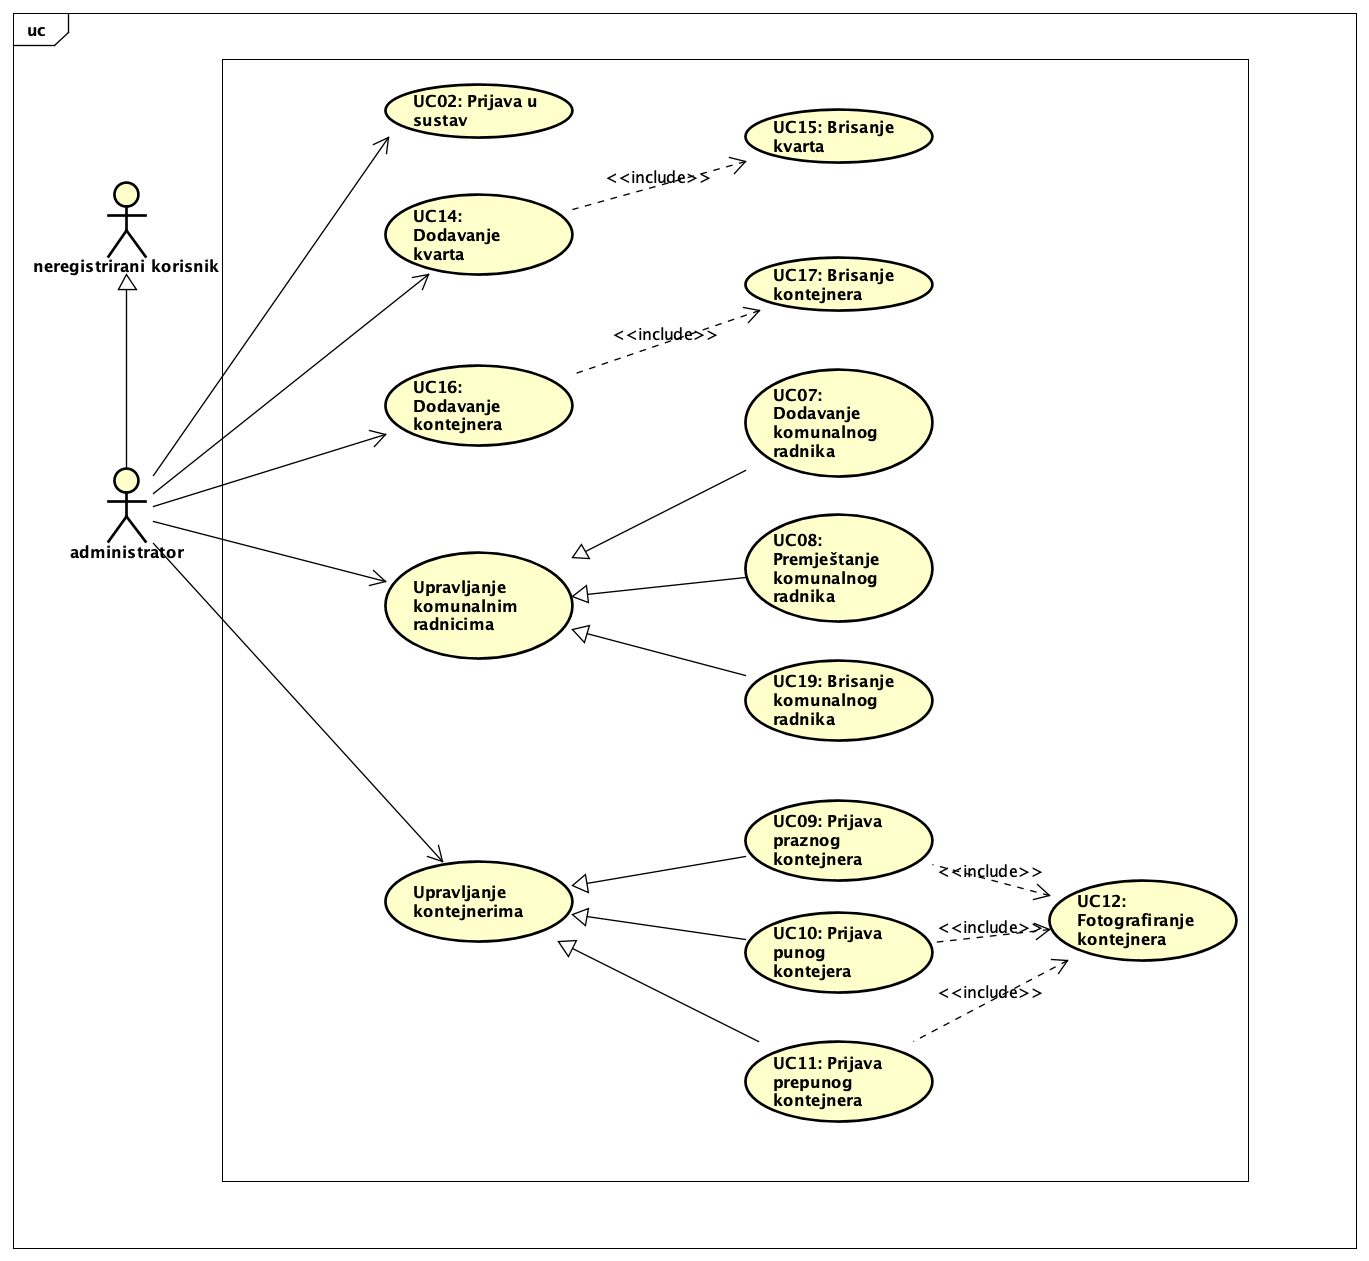
\includegraphics[scale=0.5]{figures/pravi_UC_za_administratora.PNG}
					\centering
					\caption{Dijagram obrasca uporabe, funkcionalnost administratora}
					\label{fig:ucad-diag}
				\end{figure}
			
				\begin{figure}[H]
					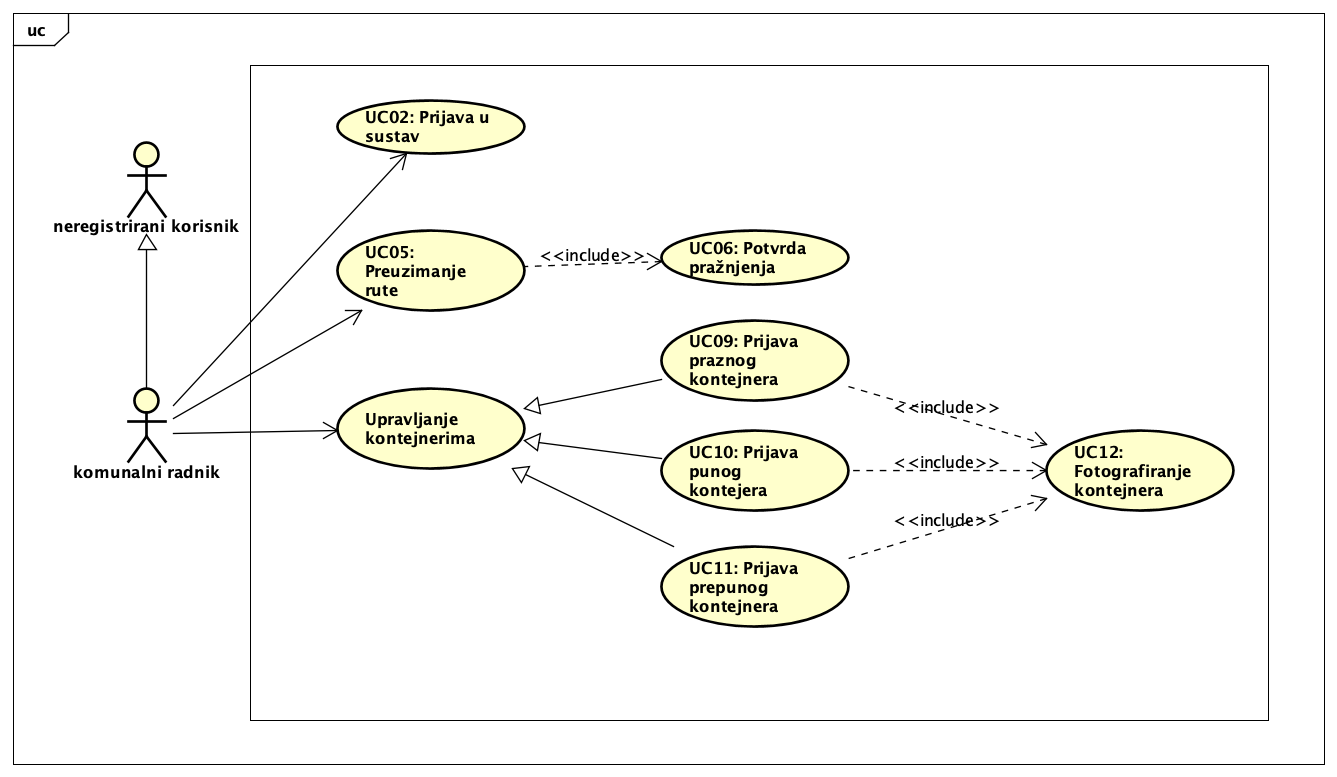
\includegraphics[scale=0.4]{figures/pravi_UC_za_smetlara.PNG}
					\centering
					\caption{Dijagram obrasca uporabe, funkcionalnost komunalnog radnika}
					\label{fig:ucad-diag}
				\end{figure}
			
				
			
				\begin{figure}[H]
					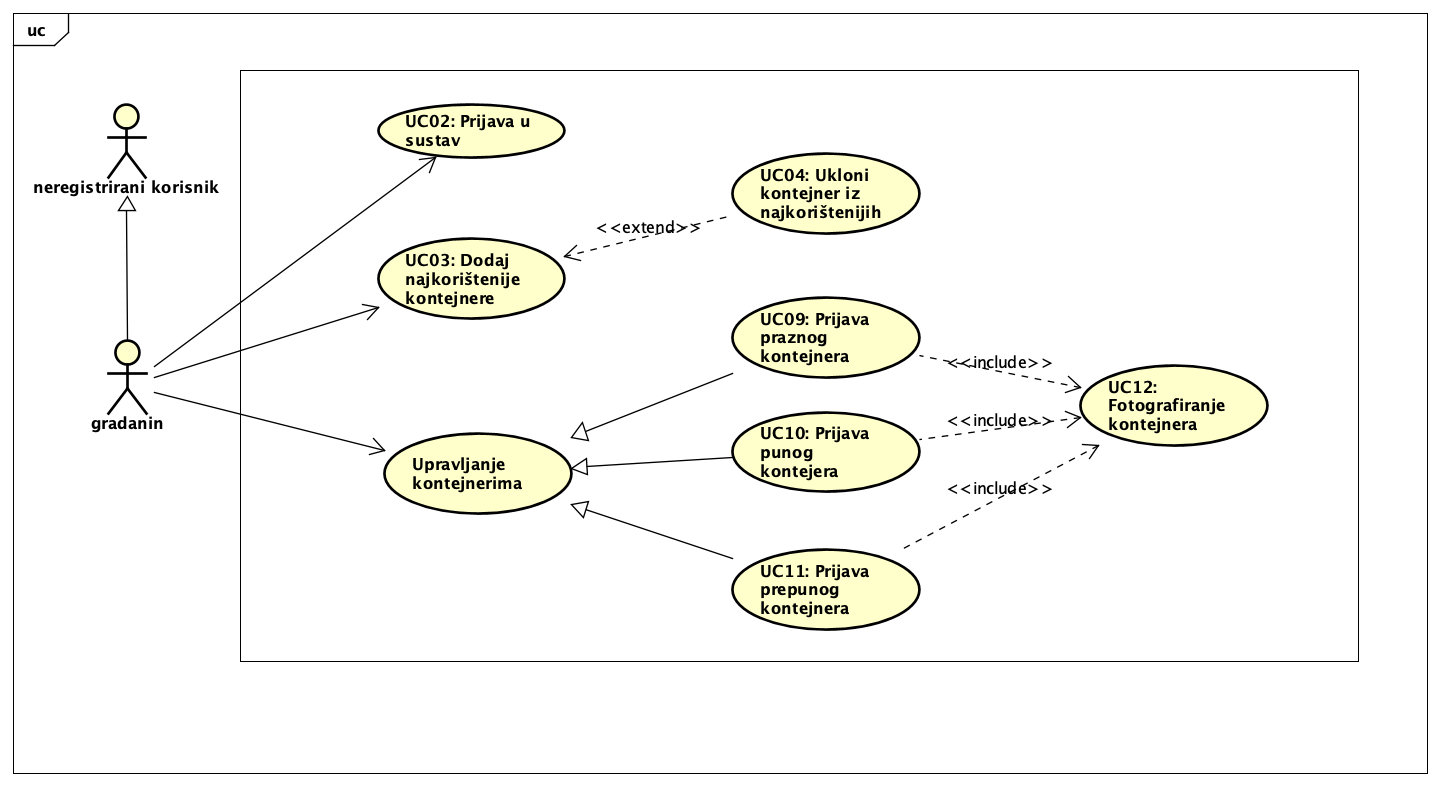
\includegraphics[scale=0.4]{figures/pravi_UC_za_gradana.PNG}
					\centering
					\caption{Dijagram obrasca uporabe, funkcionalnost građanina}
					\label{fig:ucgr-diag}
				\end{figure}
			
				

				\begin{figure}[H]
					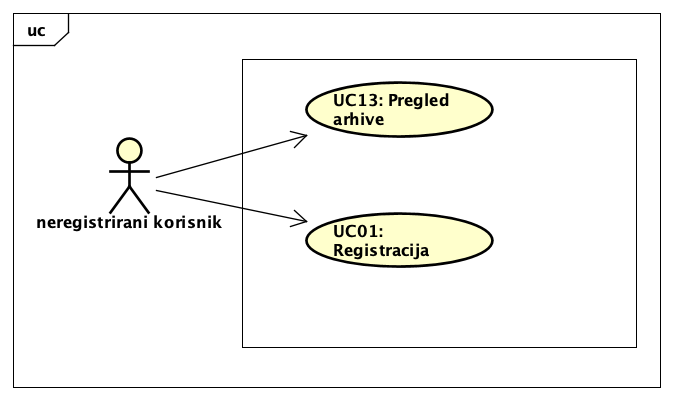
\includegraphics[scale=0.6]{figures/pravi_UC_za_neregistriranogkorisnika.PNG}
					\centering
					\caption{Dijagram obrasca uporabe, funkcionalnost neregistriranog korisnika}
					\label{fig:ucgr-diag}
				\end{figure}
			
					
					
					
					
						\eject		
				
			\subsection{Sekvencijski dijagrami}
				
				
				
				
				\noindent {\textbf{Obrazac uporabe 05 - Preuzimanje rute}}
				
				Komunalni radnik šalje zahtjev za dodjeljivanje rute kojom će prolaziti prilikom pražnjenja kontejnera u obliku popisa lokacija konterjnera koje mora isprazniti. Poslužitelj dohvaća kante u kvartu u kojem dotični komunalni radnik djeluje te mu ispiusuje onoliko kontejnera koliko stane u njegov kamion. Uzmimo za primjer kamion kapaciteta 20, dodavanjem jednog punog kontejnera na popis kapacitet se smanjuje na 19, a dodavanjem slijedećeg prepunog kontejnera smanjit će se za 2, odnosno na 20 te će ispisati onoliko kontejnera kolko stane u taj kamion.\\\\\\\\\\\\
				
				\begin{figure}[H]
					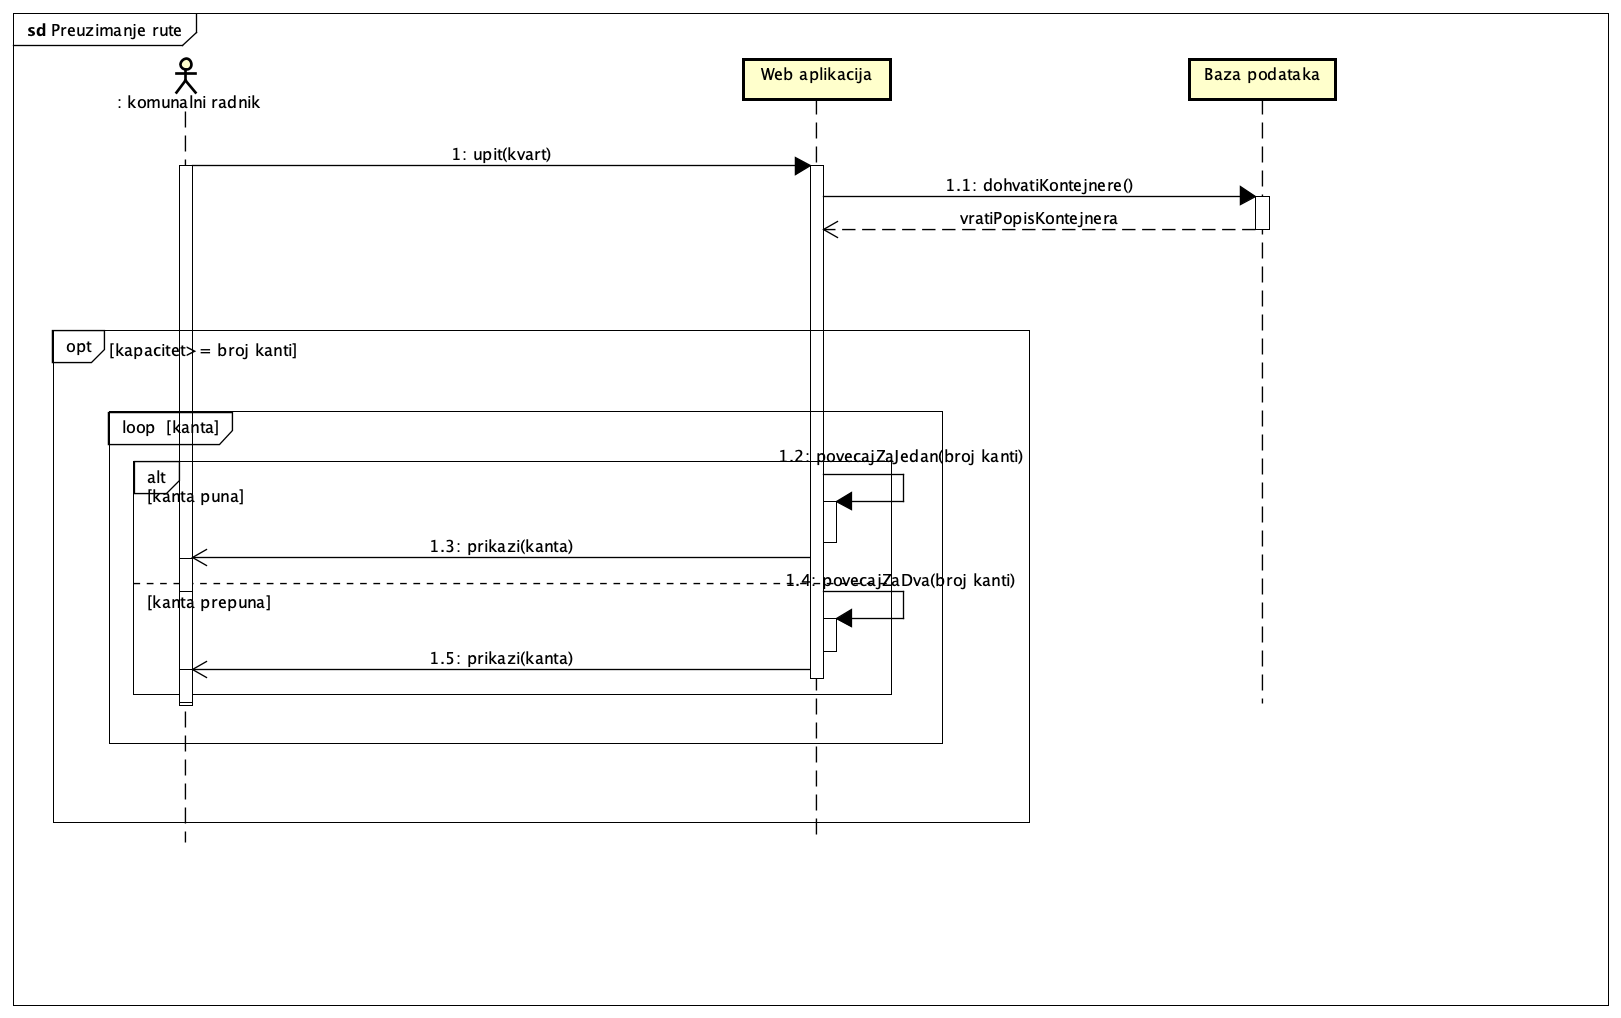
\includegraphics[scale=0.4]{figures/pravo_Preuzimanje_rute.PNG}
					\centering
					\caption{Sekvencijski dijagram za UC05}
					\label{fig:sekv-uc05}
				\end{figure}
			
							
								
				
				
				
				
				\noindent {\textbf{Obrazac uporabe 08 - Premještanje komunalnog radnika}}
				
				
				Kako bi izvršio premještaj radnika iz jednog kvartovskog poduzeća u drugo administrator mora poduzeti slijedeće; administrator bira kvart kojem je dotični radnik trenutno pridjeljen te traži u njemu istog radnika. Poslužitelj mu izlistava popis svih djelatnika u tom poduzeću te administrator bira traženog djelatnika. Poslužitelj mu izlistava informacije o tom djelatniku te mogućnosti s istim. Administrator bira premještanje te unosi željeni odredišni kvart. Ukoliko u trenutnom kvartovskom poduzeću tom akcijom neće biti premalo radnika niti u odredišnom previše poslužitelj obavlja zahtjev te dojavljuje korisniku infomaciju o uspješnom izvođenju zahtjeva. U suprotnom premještaj se neće izvršiti. \\\\
				
				\begin{figure}[H]
					\includegraphics[scale=0.5]{figures/Premještanje_komunalnog_radnika.PNG}
					\centering
					\caption{Sekvencijski dijagram za UC08}
					\label{fig:sekv-uc08}
				\end{figure}

					\noindent {\textbf{Obrazac uporabe 13 - Pregled arhive}}
				
				
				Kako bi neregesistrirani korisnik mogao pregledavati arhivu mora prvotno unijeti kvart za kojeg želi pregledati arhivu i datum. Poslužitelj mu vraća prikaz karte sa kontejnerima koji su se u tom trenutku nalazili na tom kvartu. Korisnik može odabrati pojedinu kantu te će mu poslužitelj prikazati popis svih prijava i pražnjenja tog kontejnera toga dana. \\
				
				\begin{figure}[H]
					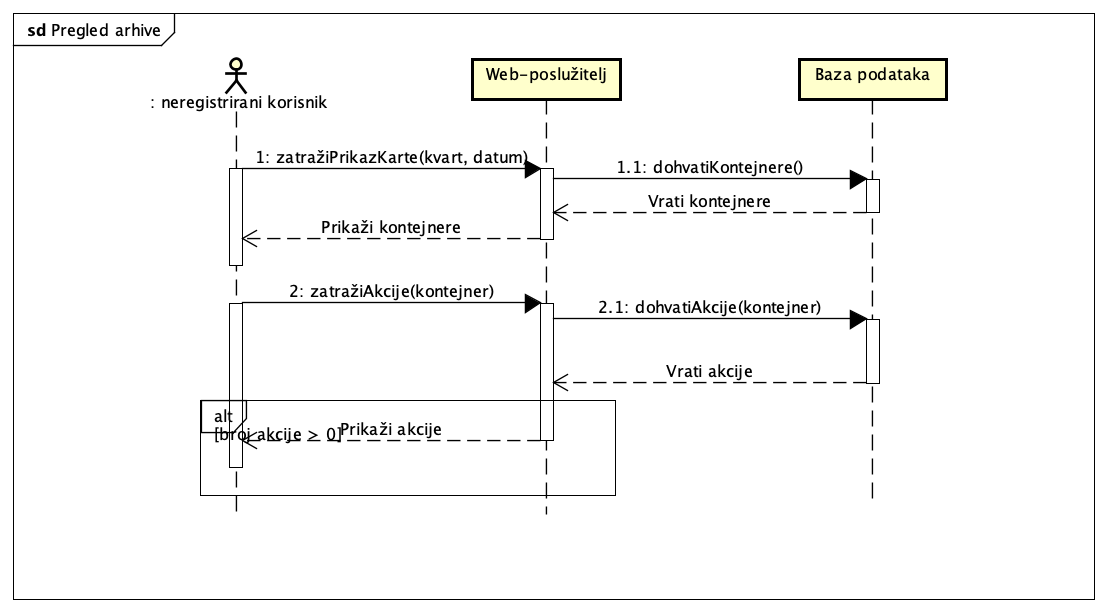
\includegraphics[scale=0.5]{figures/Pregled_arhive.PNG}
					\centering
					\caption{Sekvencijski dijagram za UC13}
					\label{fig:sekv-uc13}
				\end{figure}

				
				
				\eject
	
	
	
		\section{Ostali zahtjevi}\
		
			
	\begin{packed_item}
	
		\item {Sustav treba omogućiti rad više korisnika u stvarnom vremenu}
		\item {Sustav i korisničko sučelje trebaju podržavati dijakritičke znakove}	
		\item {Sustav treba biti implementiran kao web aplikacija koristeći objektno-orjentirane jezike}
		\item {Pristup sustavu mora biti omogućen iz javne mreže pomoću HTTPSa}
		\item {Veza uspostavljena s bazom podataka treba biti sigurna, brza i otporna na vanjske greške}
		\item {Transakcije nad bazom podataka moraju imati ograničeno trajanje}
		\item {Nadogradnja sustava ne smije narušavati postojeće funkcionalnosti sustava}
		\item {Sustav treba biti jednostavan i praktičan za korištenje}
		\item {Pogreške pri radu korisnika u korisničkom sučelju  ne smiju utjecati na ispravan rad sustava.}
	
	\end{packed_item}
		 	 
			 
			 
	